\section{Algoritmo exacto para cografo y grafo completo}

% El nuevo problema que tienen Marty y el Doc es que ahora no se ponen de
% acuerdo en qué estructura quı́mica deben utilizar para armar el condensador
% de flujos. Marty, a partir de las propiedades atómicas, ha obtenido una
% constante n y está seguro de que la solución que están buscando debe ser un
% grafo de a lo sumo n vértices (o como él lo dice, un subgrafo de algún Kn),
% mientras que el Doc ha estudiado las caracterı́sticas moleculares e insiste
% con que debe ser un subgrafo de un cografo dado. Por las dudas, y para
% evitar más conflictos entre ellos, quieren cumplir con ambas
% especificaciones, siempre maximizando la cantidad de aristas, dado que éste
% es el punto clave para su funcionamiento dentro del condensador. Por eso les
% pedimos que los ayuden diseñando e implementando un algoritmo exacto para
% MCS que tenga complejidad temporal polinomial para el caso en el que G1 es
% un cografo y G2 es un grafo completo y desarrollen los siguientes puntos que
% avalen la solución encontrada (si estamos hablando de viajar en el tiempo,
% no hay margen de error posible):
% a) Explicar detalladamente el algoritmo implementado.
% b) Calcular el orden de complejidad temporal de peor caso del algoritmo.
% c) Realizar una experimentación que permita observar los tiempos de
%    ejecución del algoritmo en función del tamaño de entrada.

\subsection{Introducción}
En este ejercicio, se busca encontrar un algoritmo exacto para resolver, en
tiempo polinomial, el problema del \acr{MCS} entre dos grafos cuando uno de
ellos es un grafo completo y el otro es un \emph{cografo}. La clase de los
cografos, o grafos reducibles por complemento, se define recursivamente y
consiste exactamente en los grafos que pueden construirse según alguna de las
siguientes reglas:
\begin{enumerate}
    \item Un nodo aislado ($K_1$) es un cografo.
    \item La unión de dos o más cografos es un cografo.
    \item El complemento de un cografo es un cografo.
\end{enumerate}

Es posible demostrar (\cite{corneil}, Corneil et al.) que todo cografo
admite una representación mediante un árbol enraizado, que se conoce como
coárbol (o \emph{cotree}) del mismo. Existen diferentes variantes de esta
representación, pero en todas ellas las hojas del árbol corresponden a los
nodos del grafo, mientras que los nodos internos representan el cografo que se
obtiene aplicando una determinada operación a los cografos relativos a sus
nodos hijos. Así, la raíz del coárbol se corresponde con el cografo completo
que se busca representar.

% Para obtener esta representación se parte de que todo cografo, o bien es una
% unión disjunta de cografos, o su complemento lo es. De esto se sigue que
% todo cografo puede reducirse a un conjunto de nodos aislados complementando
% de forma sucesiva sus componentes conexas (de allí que a estos grafos se los
% conozca como \emph{reducibles por complemento}). Esto equivale a decir que
% puede darse una forma iterativa para construir cualquier cografo a partir de
% sus nodos; se comienza considerando todos ellos como grafos disjuntos, y
% luego se conectan estos grafos iterativamente computando en cada paso el
% complemento de la unión de algunos de ellos. Dado un cografo cualquiera, su
% coárbol no es más que la representación de este proceso mediante un árbol:
% las hojas del mismo corresponden a los nodos del cografo, y cada nodo
% interno representa el complemento de la unión de los cografos
% correspondientes a sus hijos. El cografo en sí mismo es representado la raíz
% del árbol.

En este trabajo, las dos operaciones que se utilizarán para etiquetar los
nodos internos de un coárbol provienen de una definición alternativa y
equivalente de cografo: un grafo es un cografo si y solo si puede obtenerse a
partir de nodos aislados mediante la aplicación sucesiva de la unión disjunta
($\cup$) y el \emph{join} ($\times$). Esta última operación se define de la
siguiente forma: dados $G_1, \dots, G_k$ grafos, el \emph{join} entre ellos es
el grafo $G_1 \times \dots \times G_k = \left((G_1)\comp \cup
\dots \cup (G_k)\comp\right)\comp$. Una forma más intuitiva de pensar el
\emph{join} entre grafos es partir de la unión disjunta entre ellos, y agregar
todas las aristas cuyos extremos se encontraban en grafos distintos.

Otra consideración a tener en cuenta es que, para simplificar la
implementación, se utilizarán coárboles estrictamente binarios; es decir,
cada nodo interno representará una operación entre exactamente dos cografos.
Esto no resulta problemático, ya que tanto la unión como el \emph{join} entre
grafos son operaciones asociativas.

\begin{figure}[htbp]
    \centering
    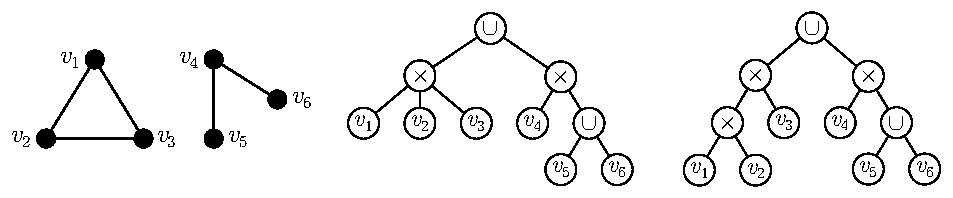
\includegraphics{imagenes/ex3_ejemplo-coarbol.pdf}
    \caption{Ejemplo de un cografo, su coárbol correspondiente, y la
    representación estrictamente binaria del mismo.}
    \label{fig:cografos:ejemplo-coarbol}
\end{figure}

\subsection{Resolución algorítmica}
Sean $G_1$ un cografo con $N_1$ nodos y $M_1$ aristas, y $G_2 = K_{N_2}$ un
grafo completo de $N_2$ nodos (que tendrá por lo tanto $M_2 = \frac{N_2 \times
(N_2 - 1)}{2}$ aristas). A la hora de resolver el problema de encontrar el
\acr {MCS} entre $G_1$ y $G_2$, pueden distinguirse estos dos casos:
\begin{enumerate}
    \item $N_1 \leq N_2$. Dado que $G_2$ es un grafo completo, todo
    subgrafo que tenga $N_2$ o menos nodos, y en particular $G_1$,
    es isomorfo a algún subgrafo de $G_2$. Como, trivialmente, $G_1$ es
    isomorfo a sí mismo, basta tomar $G_1$ como solución del problema.
    \item $N_1 > N_2$. En este caso, sea $H$ un grafo isomorfo a algún
    subgrafo de $G_1$; $H$ resultará isomorfo a algún subgrafo de $G_2$ si
    y solo si su cantidad de nodos es menor o igual que $N_2$. Si $H$ tiene
    menos de $N_2$ nodos, puede extenderse a algún grafo $\tilde{H} \supseteq
    H$ que tenga $N_2$ nodos y también sea isomorfo a un subgrafo de $G_1$.
    Es directo que $\tilde{H}$ resulta isomorfo a algún subgrafo de $G_2$ y
    que su cantidad de aristas es mayor o igual que la de $H$. Entonces, si
    $H$ era solución óptima de \acr{MCS}, claramente $\tilde{H}$ también lo
    es. De esto se sigue que para resolver este caso del problema, basta con
    tomar un subgrafo de $G_1$ que tenga exactamente $N_2$ nodos y maximice la
    cantidad de aristas.
\end{enumerate}

Dado que la resolución del primer caso es trivial, durante el resto de esta
sección se asumirá que $N_1 > N_2$. Se llamará $G = G_1$, $N = N_1$, $M = M_1$
y $K = N_2$, y se explicará la solución planteada al problema de encontrar un
subgrafo de un cografo $G$ que tenga exactamente $K$ vértices y cantidad de
aristas máxima. Aprovechando la hipótesis de que $G$ es un cografo,
es posible solucionar el problema en tiempo polinomial.

La solución propuesta tiene dos etapas. En primer lugar, se crea el coárbol
binario de $G$, y luego, utilizando la técnica de programación dinámica, se
aprovecha esta representación para obtener el subgrafo buscado.

\subsubsection{Resultados preliminares}
A continuación, se demostrarán una serie de resultados que serán necesarios
para asegurar la correctitud de los algoritmos presentados más adelante.

\begin{lema} Sea $G$ un cografo. Si $H \subseteq G$ es un subgrafo inducido de
$G$, entonces $H$ es un cografo.
\end{lema}
\begin{proof}
Por inducción estructural, utilizando la definición recursiva de cografo.
\begin{enumerate}
    \item Caso base: $G = K_1$. En este caso, necesariamente, $H = K_1$, que
    es un cografo.
    \item Caso recursivo: $G = G_1 \cup G_2$ o $G = G_1 \times G_2$, con $G_1$
    y $G_2$ cografos. Se supone, por hipótesis inductiva, que todo subgrafo
    inducido de los mismos es, a su vez, un cografo. Existen dos
    posibilidades:
    \begin{enumerate}
        \item $H \subseteq G_1$ o $H \subseteq G_2$, en cuyo caso la hipótesis
    inductiva asegura que $H$ es un cografo.
        \item Hay nodos de $H$ tanto en $G_1$ como en $G_2$. En tal caso, sean
    $H_1$ y $H_2$ los subgrafos inducidos en $G_1$ y $G_2$, respectivamente,
    por los nodos correspondientes de $H$. Por hipótesis inductiva, $H_1$ y
    $H_2$ son cografos. Notar que si $G = G_1 \cup G_2$, entonces $H = H_1
    \cup H_2$, mientras que si $G = G_1 \times G_2$, entonces $H = H_1 \times
    H_2$. En ambos casos, $H$ resulta ser un cografo. \qedhere
    \end{enumerate}
\end{enumerate}
\end{proof}

\subsubsection{Construcción del coárbol}
Para construir el coárbol correspondiente a un cografo dado, se descompone el
mismo en cografos de menor tamaño hasta obtener un conjunto de vértices
aislados. El algoritmo admite una sencilla formulación recursiva: si el
cografo consiste en un vértice aislado, el coárbol tendrá un único nodo
representando este vértice. En caso contrario, el cografo será la unión o el
\emph{join} de dos cografos; el coárbol que lo represente tendrá como raíz un
nodo etiquetado con esa operación, del cual colgarán los coárboles
correspondientes a los dos cografos sobre los cuales esta se aplica.

\bigskip
\begin{algorithm}[H]
    \SetAlgoVlined
    \caption{Construcción del coárbol correspondiente a un cografo}
    \Input{Un cografo $G = (V, E)$ con $N$ nodos y $M$ aristas, representado
    como listas de adyacencia.}
    \Output{El coárbol binario correspondiente a $G$.}

    $G\comp$ $\gets$ complemento de $G$ \;
    \textit{nodo\_inicial} $\gets$
    $\langle$subgrafo: $G$, padre: \textit{ninguno}, lado: \textit{ninguno}$\rangle$ \;
    \textit{a\_expandir} $\gets$ cola de nodos vacía \;
    \textit{a\_expandir}.encolar(\textit{nodo\_inicial}) \;

    \While{\textit{a\_expandir} no esté vacía} {
        \textit{subgrafo\_actual} $\gets$ \textit{a\_expandir}.desencolar().subgrafo \;
        \textit{padre\_actual} $\gets$ \textit{a\_expandir}.desencolar().padre \;
        \textit{lado\_actual} $\gets$ \textit{a\_expandir}.desencolar().lado \;
        $cc_1$ $\gets$ componente conexa de ($G$ restringido a) \textit{subgrafo\_actual} \;
        \eIf{$cc_1$ tiene la misma cantidad de nodos que \textit{subgrafo\_actual}} {
            $cc_1$ $\gets$ componente conexa de ($G\comp$ restringido a) el complemento de \textit{subgrafo\_actual} \;
            \textit{operación} $\gets$ $\times$ \;
        } {
            \textit{operación} $\gets$ $\cup$ \;
        }
        $cc_2$ $\gets$ \textit{subgrafo\_actual} $-$ $cc_1$ \;
        \textit{nuevo\_nodo} $\gets$ nodo representando a \textit{operación} \;
        \eIf{\textit{padre\_actual} $==$ \textit{ninguno}} {
            \textit{raíz\_cotree} $\gets$ \textit{nuevo\_nodo} \;
        } {
            \eIf{\textit{lado\_actual} $==$ \textit{izquierda}} {
                \textit{padre\_actual}.setear\_hijo\_izquierdo(\textit{nuevo\_nodo}) \;
            } {
                \textit{padre\_actual}.setear\_hijo\_derecho(\textit{nuevo\_nodo}) \;
            }
        }
        \eIf{$cc_1$ tiene exactamente 1 nodo} {
            \textit{nuevo\_nodo}.setear\_hijo\_izquierdo($cc_1$.obtener\_nodo()) \;
        } {
            \textit{a\_expandir}.encolar($\langle cc_1$, \textit{nuevo\_nodo}, \textit{izquierda}$\rangle$) \;
        }
        \eIf{$cc_2$ tiene exactamente 1 nodo} {
            \textit{nuevo\_nodo}.setear\_hijo\_derecho($cc_2$.obtener\_nodo()) \;
        } {
            \textit{a\_expandir}.encolar($\langle cc_2$, \textit{nuevo\_nodo}, \textit{derecha}$\rangle$) \;
        }
    }
    % $cotree$ $\gets$ cotree correspondiente a $G$ \;
    % $DP$ $\gets$ grilla de dimensiones $(2 \times N - 1) \times K$, donde
    % cada fila representa a uno de los vértices del coárbol de $G$, y cada
    % columna,
    \Return{\textit{raíz\_cotree}}
\end{algorithm}
\bigskip

\subsubsection{Búsqueda del subgrafo máximo}
Para encontrar el subgrafo de $G$ con $K < N$ nodos y máxima cantidad de
aristas, se diseñó un algoritmo utilizando la técnica de programación
dinámica. El esquema detrás de la formulación recursiva de este algoritmo es
el siguiente:

\begin{enumerate}
    \item Si $K = 0$, la solución del algoritmo es un grafo sin nodos ni
    aristas.
    \item Si $K > 0$ y $G = K_1$, es decir, un nodo aislado, la solución es
    $K_1$.
    \item Si $G \neq K_1$, entonces existen dos cografos $G_1$ y $G_2$ tales
    que $G = G_1 \times G_2$ o $G = G_1 \cup G_2$. En tal caso, la solución
    $H$ del problema tendrá algunos de sus nodos en $G_1$ y el resto en $G_2$.
    Entonces, según la operación con la que se obtenga $G$ a partir de $G_1$ y
    $G_2$, tenemos que $H = H_1 \times H_2$ o $H = H_1 \cup H_2$, donde
    $H_1$ y $H_2$ son los subgrafos inducidos en $G$ por los nodos de $H$ que
    pertenecen a $G_1$ y a $G_2$, respectivamente.
\end{enumerate}

\[
    \operatorname{MCS}(G, K) = \begin{cases}
        (\varnothing, \varnothing) & \text{si } K = 0 \\
        K_1 & \text{si } G \text{ es un nodo aislado} \\
        \displaystyle \argmax_{H \in S(G, K)}(\#E(H)) & \text{si } G = (G_1
        \cup G_2) \text{ o } G = (G_1 \times G_2) \\
    \end{cases}
\]

donde

\[
    S(G, K) = \begin{cases}
        \lbrace \operatorname{MCS}(G_1, k) \cup \operatorname{MCS}(G_2, K -
        k) \ \vert\ 0 \leq k \leq \#V(G_1) \rbrace & \text{si } G = (G_1 \cup G_2) \\
        \lbrace \operatorname{MCS}(G_1, k) \times \operatorname{MCS}(G_2, K -
        k) \ \vert\ 0 \leq k \leq \#V(G_1) \rbrace & \text{si } G = (G_1 \times G_2)
    \end{cases}
\]

\bigskip
\begin{algorithm}[H]
    \caption{Subgrafo máximo de un cografo}
    \Input{Un cografo $G = (V, E)$ con $N$ nodos y $M$ aristas, y un natural
        $K < N$.}
    \Output{Un subgrafo $H \subseteq G$ con $K$ nodos que maximice la cantidad
        de aristas.}

    $cotree$ $\gets$ coárbol correspondiente a $G$ \;
    $DP$ $\gets$ grilla de dimensiones $(2 \times N - 1) \times K$, donde \;
    cada fila representa a uno de los vértices del coárbol de $G$, y cada \;
    columna,
    \Return{($DP_{N,M}$, $camino$)}
\end{algorithm}
\bigskip

El algoritmo planteado para la búsqueda del máximo subgrafo


\subsection{Detalles implementativos}

\subsection{Complejidad}
Defino $N_1$ la cantiadad de nodos de $g_1$ (cografo) y $M_1$ la cantiadad de aristas,
$N_2$ la cantidad de nodos del $g_2$ ($K_n$)

Armar el coárbol tiene una complejidad $\ord(N_1(N_1 + M_1))$, hacer el DP que
calcula la solucion $\ord(N_1 * (N_2)^2 )$

En total el algoritmo termina teniendo una complejidad de $\ord(N_1((N_1 + M_1) + (N_2)^2 ))$

\subsection{Experimentación}
Una vez completada la implementación del algoritmo, se realizaron pruebas
experimentales con el fin de corroborar la cota teórica calculada para la
complejidad temporal del mismo.

Con el fin de tener un mejor control de las variables involucradas, se
experimentó por separado con la creación del coárbol y con la resolución del
algoritmo de programación dinámica, teniendo en cuenta que ambas etapas se
ejecutan de forma sucesiva y que, de cumplir ambas con la cota teórica
correspondiente a cada una de ellas, esto implica que el algoritmo completo
también cumplirá con su respectiva cota.


\begin{enumerate}
    \item Para la creación del coarbol, los tres experimentos realizados son:
    \begin{enumerate}
        \item \label{ex3:coarbol_union_k1} Se toma como $G_1$ la unión
        disjunta de $K_1$, con lo cual se fija la cantidad de aristas en $0$
        ($M_1$), y se varía la cantidad de nodos del cografo ($N_1$). Se
        espera así mostrar que la complejidad es de orden cuadrático con
        respecto a $N_1$.
        \item \label{ex3:coarbol_union_k3} Se toma como $G_1$ la unión
        disjunta de $K_3$; cada 3 nuevos nodos hay 3 nuevas aristas, logrando
        una relación lineal $M_1 = N_1$. Se espera un crecimiento cuadrático
        con respecto a $N_1$ con una constante más alta que la unión de $K_1$,
        con lo cual se quiere probar parcialmente la influencia de $M_1$ y
        confirmar la dependencia cuadrática respecto de $N_1$.
        \item \label{ex3:coarbol_kn} Se toma un $K_{N_1}$, con lo cual se
        tiene una relación cuadrática $M_1 = \frac{N_1(N_1 - 1)}{2} =
        \ord(N^2)$. Se espera una complejidad cuadrática con respecto a $N_1$,
        con la cual se pretende mostrar la influencia de $M_2$.
    \end{enumerate}

    \item Para la resolución del algoritmo de DP, los tres experimentos
    realizados son:
    \begin{enumerate}
        \item \label{ex3:dp_n2_const} Se varían los nodos del cografo ($N_1$) y se
        fija el $K_N$ ($G_2$) en 100 nodos. Se varía la cantidad de aristas
        del cografo para ver como afecta al algoritmo de DP. Se esperan
        complejidades de orden lineal en $N_1$ difiriendo en una constante,
        dependiendo de como esté conectado el cografo. Con este experimento se
        quiere probar la dependencia lineal respecto de $N_1$.
        \item \label{ex3:dp_n2_lineal} Se varían los nodos del cografo
        ($N_1$), siendo el cografo un $K_ {N_1}$, y tomando para el segundo
        grafo $N_2 = \frac{N_1}{2}$. Se espera una complejidad de orden cúbico
        con respecto a $N_1$, con lo cual se quiere mostrar la dependencia
        cuadrática respecto de $N_2$ y confirmar la dependencia lineal
        respecto de $N_1$.
        \item \label{ex3:dp_n2_log} Se varían los nodos del cografo ($N_1$),
        siendo el cografo un $K_ {N_1}$, y tomando para el segundo grafo $N_2
        = \log_2(N_1)$. Se espera una complejidad de $\ord(N_1 \log^2(N_1))$,
        con la cual se pretende mostrar la dependencia cuadrática respecto de
        $N_2$ y confirmar la dependencia lineal de $N_1$.
    \end{enumerate}
\end{enumerate}

\subsubsection{Experimentos con la creación del coárbol}


\paragraph{Experimento \ref{ex3:coarbol_union_k1}}
Se ejecuta la creación del coárbol, siendo $G_1$ una unión disjunta de grafos
triviales. Se fija la cantidad de aristas ($M_1$) en $0$ y se varia la
cantidad de nodos del cografo ($N_1$). Como $M_1 = 0$, queda una complejidad
$\ord(N_1(N_1 + 0))$ = $\ord(N_1^2)$.

\begin{figure}[H]
    \centering
    \begin{tikzpicture}
        \begin{axis}[
                title={},
                xlabel={Cantidad de nodos del cografo ($N_1$)},
                ylabel={Tiempo de ejecución (nanosegundos)},
                scaled x ticks=false,
                scaled y ticks=false,
                enlargelimits=0.05,
                width=0.5\textwidth,
                height=0.5\textwidth,
                legend pos=outer north east,
                legend cell align=left,
                xmin=0
            ]
            \addplot[color=black] table[x index=0,y index=1]
                {../exp/ej3/cograph_k1_union_create_cotree};
            \addplot[color=red] table[x index=0, y expr={ 12 * (x*x) }]
                {../exp/ej3/cograph_k1_union_create_cotree};
            \legend{$T_{K_1}$, $c * N_1^2$ ($c = 12$)}
        \end{axis}
    \end{tikzpicture}
    \caption{Resultados obtenidos para el experimento \ref{ex3:coarbol_union_k1}}
    \label{fig:exp3:var-nym-base}
\end{figure}

Se divide por $N_1^2$, para mostrar la validez de la cota teórica.
\begin{figure}[H]
    \centering
    \begin{tikzpicture}
        \begin{axis}[
                title={},
                xlabel={Cantidad de nodos del cografo ($N_1$)},
                ylabel={Tiempo de ejecución (nanosegundos) / $N_1^2$},
                scaled x ticks=false,
                scaled y ticks=false,
                enlargelimits=0.05,
                width=0.5\textwidth,
                height=0.5\textwidth,
                legend pos=outer north east,
                legend cell align=left,
                xmin=0,
                ymax= 50
            ]
            \addplot[color=black] table[x index=0,y expr={\thisrowno{1}/(x*x)}]
                {../exp/ej3/cograph_k1_union_create_cotree};
            \addplot[color=red] table[x index=0, y expr={ 12 }]
                {../exp/ej3/cograph_k1_union_create_cotree};
            \legend{$T_{K_1}/N_1^2$, $c = 12$}
        \end{axis}
    \end{tikzpicture}
    \caption{Resultados del experimento \ref{ex3:coarbol_union_k1}, dividiendo
    por la cota de complejidad teórica}
    \label{fig:exp3:var-nym-base}
\end{figure}

\paragraph{Experimento \ref{ex3:coarbol_union_k3}}
Se ejecuta la creación del coárbol, siendo $G_1$ una unión disjunta de $K_3$.
Como $M_1 = N_1$, queda una complejidad $\ord(N_1(N_1 + N_1))$ = $\ord(N_1^2)$.

\begin{figure}[H]
    \centering
    \begin{tikzpicture}
        \begin{axis}[
                title={},
                xlabel={Cantidad de nodos del cografo ($N_1$)},
                ylabel={Tiempo de ejecución (nanosegundos)},
                scaled x ticks=false,
                scaled y ticks=false,
                enlargelimits=0.05,
                width=0.5\textwidth,
                height=0.5\textwidth,
                legend pos=outer north east,
                legend cell align=left,
                xmin=0
            ]
            \addplot[color=black] table[x index=0,y index=1]
                {../exp/ej3/cograph_k3_union_create_cotree};
            \addplot[color=red] table[x index=0, y expr={  140 * (x*x) }]
                {../exp/ej3/cograph_k3_union_create_cotree};
            \legend{$T_{K_3}$,$ c * N_1^2 $ ($c = 140$)}
        \end{axis}
    \end{tikzpicture}
    \caption{Resultados del experimento \ref{ex3:coarbol_union_k3}}
    \label{fig:exp3:var-nym-base}
\end{figure}

Se divide por $N_1^2$, para mostrar que $c = 140$ lo acota.

\begin{figure}[H]
    \centering
    \begin{tikzpicture}
        \begin{axis}[
                title={},
                xlabel={Cantidad de nodos del cografo ($N_1$)},
                ylabel={Tiempo de ejecución (nanosegundos) / $N_1^2$},
                scaled x ticks=false,
                scaled y ticks=false,
                enlargelimits=0.05,
                width=0.5\textwidth,
                height=0.5\textwidth,
                legend pos=outer north east,
                legend cell align=left,
                xmin=0,
                ymax= 200
            ]
            \addplot[color=black] table[x index=0,y expr={\thisrowno{1}/(x*x)}]
                {../exp/ej3/cograph_k3_union_create_cotree};
            \addplot[color=red] table[x index=0, y expr={140}]
                {../exp/ej3/cograph_k3_union_create_cotree};
            \legend{$T_{K_3}/N_1^2$,$ c = 140 $}
        \end{axis}
    \end{tikzpicture}
    \caption{Resultados del experimento \ref{ex3:coarbol_union_k3}, dividiendo
    por la cota de complejidad teórica}
    \label{fig:exp3:var-nym-base}
\end{figure}


\paragraph{Experimento \ref{ex3:coarbol_kn}}
Se ejecuta la creación del coárbol, siendo $G_2$ un completo de $N_1$ nodos.
Como $M_1 = \frac{N_1(N_1 - 1)}{2} = \frac{N_1^2 - N_1}{2}$, queda una complejidad
$\ord(N_1(N_1 + \frac{N_1^2 - N_1}{2}))$ = $\ord(N_1^3)$.

\begin{figure}[H]
    \centering
    \begin{tikzpicture}
        \begin{axis}[
                title={},
                xlabel={Cantidad de nodos del cografo ($N_1$)},
                ylabel={Tiempo de ejecución (nanosegundos)},
                scaled x ticks=false,
                scaled y ticks=false,
                enlargelimits=0.05,
                width=0.5\textwidth,
                height=0.5\textwidth,
                legend pos=outer north east,
                legend cell align=left,
                xmin=0
            ]
            \addplot[color=black] table[x index=0,y index=1]
                {../exp/ej3/cograph_kn_create_cotree};
            \addplot[color=red] table[x index=0, y expr={ 17 * (x*x*x) }]
                {../exp/ej3/cograph_kn_create_cotree};
            \legend{$T_{K_{N_1}}$, $c * N_1^3$ ($c=17$))}
        \end{axis}
    \end{tikzpicture}
    \caption{Resultados del experimento \ref{ex3:coarbol_kn}}
    \label{fig:exp3:var-nym-base}
\end{figure}

Se divide por $N_1^3$, para mostrar que $c = 17$ lo acota.

\begin{figure}[H]
    \centering
    \begin{tikzpicture}
        \begin{axis}[
                title={},
                xlabel={Cantidad de nodos del cografo ($N_1$)},
                ylabel={Tiempo de ejecución (nanosegundos) / $N_1^3$},
                scaled x ticks=false,
                scaled y ticks=false,
                enlargelimits=0.05,
                width=0.5\textwidth,
                height=0.5\textwidth,
                legend pos=outer north east,
                legend cell align=left,
                xmin=0,
                ymax= 50
            ]
            \addplot[color=black] table[x index=0,y expr={\thisrowno{1}/(x*x*x)}]
                {../exp/ej3/cograph_kn_create_cotree};
            \addplot[color=red] table[x index=0, y expr={ 17 }]
                {../exp/ej3/cograph_kn_create_cotree};
            \legend{$T_{K_{N_1}}/N_1^3$, $c = 17$}
        \end{axis}
    \end{tikzpicture}
    \caption{Resultados del experimento \ref{ex3:coarbol_kn}, dividiendo
    por la cota de complejidad teórica}
    \label{fig:exp3:var-nym-base}
\end{figure}


\subsubsection{Experimentos con la resolución del algoritmo de DP}

\paragraph{Experimento \ref{ex3:dp_n2_const}}
Se ejecutó la resolución del DP. Como $N_2 = 100$, queda una complejidad $\ord
(N_1* 100^2)$ = $\ord(N_1)$.
Se varían los nodos del cografo ($N_1$) y se fija el $K_N$ en $100$ nodos.

\begin{figure}[H]
    \centering
    \begin{tikzpicture}
        \begin{axis}[
                title={},
                xlabel={Cantidad de nodos del cografo ($N_1$)},
                ylabel={Tiempo de ejecución (nanosegundos)},
                scaled x ticks=false,
                scaled y ticks=false,
                enlargelimits=0.05,
                width=0.5\textwidth,
                height=0.5\textwidth,
                legend pos=outer north east,
                legend cell align=left,
                xmin=100
            ]
            \addplot[color=black] table[x index=0,y index=1]
                {../exp/ej3/cograph_kn_dp};
            \addplot[color=blue] table[x index=0,y index=1]
                {../exp/ej3/cograph_k1_union_dp};
            \addplot[color=violet] table[x index=0,y index=1]
                {../exp/ej3/cograph_k10_union_dp};
            \addplot[color=red] table[x index=0, y expr={ 500000 * (x) }]
                {../exp/ej3/cograph_kn_dp};
            \legend{$T_{k_n}$,$T_{k_1}$,$T_{k_{10}}$,$ c * N_1 $ ($c = 5
            \times 10^5$)}
        \end{axis}
    \end{tikzpicture}
    \caption{Resultados del experimento \ref{ex3:dp_n2_const}}
    \label{fig:exp3:var-nym-base}
\end{figure}

Se puede ver que la constante depende del la familia del grafo;
$T_{K_{N_1}}$ y $T_{K_1}$ tiene una constante muy parecida, ya que uno es el
complemento del otro. Queda probar con diversas familias de cografos para ver
cómo afecta al la creación de coarboles. Se puede esperar que, mientras menos
balanceado sea el coarbol, más grande sera la constante, ya que en cada paso
tendría que probar hijos izquierdos por hijos derechos en el DP.

Se divide por $N_1$, para mostrar que $c = 500000$ lo acota.

\begin{figure}[H]
    \centering
    \begin{tikzpicture}
        \begin{axis}[
                title={},
                xlabel={Cantidad de nodos del cografo ($N_1$)},
                ylabel={Tiempo de ejecución (nanosegundos) / $N_1$},
                scaled x ticks=false,
                scaled y ticks=false,
                enlargelimits=0.05,
                width=0.5\textwidth,
                height=0.5\textwidth,
                legend pos=outer north east,
                legend cell align=left,
                xmin=100
            ];
            \addplot[color=black] table[x index=0,y expr={\thisrowno{1}/(x)} ]
                {../exp/ej3/cograph_kn_dp};
            \addplot[color=blue] table[x index=0,y expr={\thisrowno{1}/(x)} ]
                {../exp/ej3/cograph_k1_union_dp};
            \addplot[color=violet] table[x index=0,y expr={\thisrowno{1}/(x)} ]
                {../exp/ej3/cograph_k10_union_dp};
            \addplot[color=red] table[x index=0, y expr={ 500000 }]
                {../exp/ej3/cograph_kn_dp};
            \legend{$T_{K_{N_1}}/N_1$,$T_{K_1}/N_1$,$T_{K_{10}}/N_1$,$c = 5
            \times 10^5$}
        \end{axis}
    \end{tikzpicture}
    \caption{Resultados del experimento \ref{ex3:dp_n2_const}, dividiendo
    por la cota de complejidad teórica}
    \label{fig:exp3:var-nym-base}
\end{figure}

\paragraph{Experimento \ref{ex3:dp_n2_lineal}}
Se varían los nodos del cografo, siendo $G_1$ un $K_{N_1}$ y el segundo grafo
un completo con la mitad de nodos.

Se ejecuta la resolución del DP. Como $N_2 = \frac{N_1}{2}$, queda una
complejidad $\ord(N_1 \times (\frac{N_1}{2})^2)$ = $\ord(N_1^3)$.

\begin{figure}[H]
    \centering
    \begin{tikzpicture}
        \begin{axis}[
                title={},
                xlabel={Cantidad de nodos del cografo ($N_1$)},
                ylabel={Tiempo de ejecución (nanosegundos)},
                scaled x ticks=false,
                scaled y ticks=false,
                enlargelimits=0.05,
                width=0.5\textwidth,
                height=0.5\textwidth,
                legend pos=outer north east,
                legend cell align=left,
                xmin=0
            ]
            \addplot[color=black] table[x index=0,y index=1]
                {../exp/ej3/cograph_kn_and_k_n_div_2_dp};
            \addplot[color=red] table[x index=0, y expr={ 10 * (x*x*x) }]
                {../exp/ej3/cograph_kn_and_k_n_div_2_dp};
            \legend{$T_{K_N}$, $c * N_1^3$ ($c = 10$)}
        \end{axis}
    \end{tikzpicture}
    \caption{Resultados obtenidos para el experimento \ref{ex3:dp_n2_lineal}}
    \label{fig:exp3:var-nym-base}
\end{figure}

Se divide por $N_1^2$, para mostrar, que $c = 10$ lo acota.

\begin{figure}[H]
    \centering
    \begin{tikzpicture}
        \begin{axis}[
                title={},
                xlabel={Cantidad de nodos del cografo ($N_1$)},
                ylabel={Tiempo de ejecución (nanosegundos) / $N_1^2$},
                scaled x ticks=false,
                scaled y ticks=false,
                enlargelimits=0.05,
                width=0.5\textwidth,
                height=0.5\textwidth,
                legend pos=outer north east,
                legend cell align=left,
                xmin=0
            ]
            \addplot[color=black] table[x index=0,y expr={\thisrowno{1}/(x*x*x)}]
                {../exp/ej3/cograph_kn_and_k_n_div_2_dp};
            \addplot[color=red] table[x index=0, y expr={ 10}]
                {../exp/ej3/cograph_kn_and_k_n_div_2_dp};
            \legend{$T_{K_{N_1/2}} / N_1^2$, $c = 10$}
        \end{axis}
    \end{tikzpicture}
    \caption{Resultados del experimento \ref{ex3:dp_n2_lineal},
    dividiendo por la cota de complejidad teórica}
    \label{fig:exp3:var-nym-base}
\end{figure}

\paragraph{Experimento \ref{ex3:dp_n2_log}}
Se varía la cantidad de nodos del cografo $G_1$ ($N_1$), siendo el cografo un
$K_{N_1}$ y el segundo grafo un $K_{N_2}$ con $N_2 = \log_2(N_1)$. Se ejecuta
la resolución del DP. Como $N_2 = \log_2(N_1)$, queda una complejidad $\ord
(N_1 \times \ln^2(N_1))$.

\begin{figure}[H]
    \centering
    \begin{tikzpicture}
        \begin{axis}[
                title={},
                xlabel={Cantidad de nodos del cografo ($N_1$)},
                ylabel={Tiempo de ejecución (nanosegundos)},
                scaled x ticks=false,
                scaled y ticks=false,
                enlargelimits=0.05,
                width=0.5\textwidth,
                height=0.5\textwidth,
                legend pos=outer north east,
                legend cell align=left,
                xmin=0
            ]
            \addplot[color=black] table[x index=0,y index=1]
                {../exp/ej3/cograph_kn_and_k_log_n_dp};
            \addplot[color=red] table[x index=0, y expr={ 135 * x * ln(x) * ln(x) }]
                {../exp/ej3/cograph_kn_and_k_log_n_dp};

            \legend{$T_{K_{\log_2(N_1)}}$, $c \times N_1 \times \ln^2(N_1)$ ($c
            = 135$)}
        \end{axis}
    \end{tikzpicture}
    \caption{Resultados obtenidos para el experimento \ref{ex3:dp_n2_log}}
    \label{fig:exp3:var-nym-base}
\end{figure}

Se divide por $N_1$, para mostrar que $c \times \ln^2(N_1)$ lo acota.

\begin{figure}[H]
    \centering
    \begin{tikzpicture}
        \begin{axis}[
                title={},
                xlabel={Cantidad de nodos del cografo ($N_1$)},
                ylabel={Tiempo de ejecución (nanosegundos) / $N_1$},
                scaled x ticks=false,
                scaled y ticks=false,
                enlargelimits=0.05,
                width=0.5\textwidth,
                height=0.5\textwidth,
                legend pos=outer north east,
                legend cell align=left,
                xmin=0
            ]
            \addplot[color=black] table[x index=0,y expr={\thisrowno{1}/(x)}]
                {../exp/ej3/cograph_kn_and_k_log_n_dp};
            \addplot[color=red] table[x index=0, y expr={ 135 * ln(x) * ln(x)  }]
                {../exp/ej3/cograph_kn_and_k_log_n_dp};
            \legend{$T_{K_{\log_2(N_1)}} / N_1$, $c * \ln^2(N_1)$ ($c = 134$)}
        \end{axis}
    \end{tikzpicture}
    \caption{Resultados obtenidos para el experimento \ref{ex3:dp_n2_log},
    dividiendo por la cantidad de nodos del cografo}
    \label{fig:exp3:var-nym-base}
\end{figure}

Se divide por $N_1 * \ln^2(N_1)$, para mostrar que $c = 135$ lo acota.

\begin{figure}[H]
    \centering
    \begin{tikzpicture}
        \begin{axis}[
                title={},
                xlabel={Cantidad de nodos del cografo ($N_1$)},
                ylabel={Tiempo de ejecución (nanosegundos) / $N_1 * \ln^2(N_1)$},
                scaled x ticks=false,
                scaled y ticks=false,
                enlargelimits=0.05,
                width=0.5\textwidth,
                height=0.5\textwidth,
                legend pos=outer north east,
                legend cell align=left,
                xmin=0
            ]

            \addplot[color=black] table[x index=0,y expr={\thisrowno{1}/(x * ln(x) * ln(x)) }]
                {../exp/ej3/cograph_kn_and_k_log_n_dp};
            \addplot[color=red] table[x index=0, y expr={ 135 }]
                {../exp/ej3/cograph_kn_and_k_log_n_dp};
            \legend{$T_{K_{\log_2(N_1)}} / N_1 * \ln^2(N_1)$, $c = 135$}
        \end{axis}
    \end{tikzpicture}
    \caption{Resultados del experimento \ref{ex3:dp_n2_log},
    dividiendo por la cota de complejidad teórica}
    \label{fig:exp3:var-nym-base}
\end{figure}

\subsubsection{Conclusiones}

Como se puede observar en las conclusiones extraidas de cada experimento
particular, el conjunto de pruebas realizadas permite corroborar de forma
independiente las cotas teóricas propuestas para cada una de las etapas del
algoritmo. En su conjunto, estas dos cotas permiten verificar que la
complejidad total del algoritmo es, como se había demostrado previamente, de
$\ord(N_1(N_1 + M_1)) + \ord(N_1 \times (N_2)^2 )$ = $\ord(N_1((N_1 + M_1)
+ (N_2)^2))$.




















